\documentclass[12pt, notitlepage, final]{article} 

\newcommand{\name}{Vince Coghlan}

\usepackage{amsfonts}
\usepackage{amssymb}
\usepackage{amsmath}
\usepackage{latexsym}
\usepackage{enumerate}
\usepackage{amsthm}
\usepackage{nccmath}
\usepackage{setspace}
\usepackage[pdftex]{graphicx}
\usepackage{epstopdf}
\usepackage[siunitx]{circuitikz}
\usepackage{tikz}
\usepackage{float}
\usepackage{cancel} 
\usepackage{setspace}
\usepackage{overpic}
\usepackage{mathtools}
\usepackage{listings}
\usepackage{color}
\usepackage{pgfplots}
\pgfplotsset{legend style={line width=1pt}}


\numberwithin{equation}{section}
\DeclareRobustCommand{\beginProtected}[1]{\begin{#1}}
\DeclareRobustCommand{\endProtected}[1]{\end{#1}}
\newcommand{\dbr}[1]{d_{\mbox{#1BR}}}
\newtheorem{lemma}{Lemma}
\newtheorem*{corollary}{Corollary}
\newtheorem{theorem}{Theorem}
\newtheorem{proposition}{Proposition}
\theoremstyle{definition}
\newtheorem{define}{Definition}
\newcommand{\column}[2]{
\left( \begin{array}{ccc}
#1 \\
#2
\end{array} \right)}

\newdimen\digitwidth
\settowidth\digitwidth{0}
\def~{\hspace{\digitwidth}}

\setlength{\parskip}{1pc}
\setlength{\parindent}{0pt}
\setlength{\topmargin}{-3pc}
\setlength{\textheight}{9.0in}
\setlength{\oddsidemargin}{0pc}
\setlength{\evensidemargin}{0pc}
\setlength{\textwidth}{6.5in}
\newcommand{\answer}[1]{\newpage\noindent\framebox{\vbox{{\bf CSCI 3753 Spring 2014} 
\hfill {\bf \name} \vspace{-1cm}
\begin{center}{Programming Assignment \#3}\end{center} } }\bigskip }

%absolute value code
\DeclarePairedDelimiter\abs{\lvert}{\rvert}%
\DeclarePairedDelimiter\norm{\lVert}{\rVert}
\makeatletter
\let\oldabs\abs
\def\abs{\@ifstar{\oldabs}{\oldabs*}}
%
\let\oldnorm\norm
\def\norm{\@ifstar{\oldnorm}{\oldnorm*}}
\makeatother

\def\dbar{{\mathchar'26\mkern-12mu d}}
\def \Frac{\displaystyle\frac}
\def \Sum{\displaystyle\sum}
\def \Int{\displaystyle\int}
\def \Prod{\displaystyle\prod}
\def \P[x]{\Frac{\partial}{\partial x}}
\def \D[x]{\Frac{d}{dx}}
\newcommand{\PD}[2]{\frac{\partial#1}{\partial#2}}
\newcommand{\PF}[1]{\frac{\partial}{\partial#1}}
\newcommand{\DD}[2]{\frac{d#1}{d#2}}
\newcommand{\DF}[1]{\frac{d}{d#1}}
\newcommand{\fix}[2]{\left(#1\right)_#2}
\newcommand{\ket}[1]{|#1\rangle}
\newcommand{\bra}[1]{\langle#1|}
\newcommand{\braket}[2]{\langle #1 | #2 \rangle}
\newcommand{\bopk}[3]{\langle #1 | #2 | #3 \rangle}
\newcommand{\Choose}[2]{\displaystyle {#1 \choose #2}}
\newcommand{\proj}[1]{\ket{#1}\bra{#1}}
\def\del{\vec{\nabla}}
\newcommand{\avg}[1]{\langle#1\rangle}
\newcommand{\piecewise}[4]{\left\{\beginProtected{array}{rl}#1&:#2\\#3&:#4\endProtected{array}\right.}
\newcommand{\systeme}[2]{\left\{\beginProtected{array}{rl}#1\\#2\endProtected{array}\right.}
\def \KE{K\!E}
\def\Godel{G$\ddot{\mbox{o}}$del}

\onehalfspacing

\begin{document}

\answer{}

\section{Abstract}

\section{Introduction}
A scheduler is a vital part of any modern operating system.  It decides how to efficiently
utilize the CPU.  This is important in the resource manager view of an operating system,
that the OS is only supposed to manage resources.  There are three schedulers that I will
test, the Completely Fair Scheduler(CFS), also known as SCHED\_OTHER, the First in First
Out(FIFO) scheduler, also known as SCHED\_FIFO, and the Round Robin(RR) Scheduler, also
known as SCHED\_RR.

Every test was preformed on a Macbook Pro running Ubuntu 12.04 through VMWare Fusion.
The VM has 2Gb of RAM, 2 Cores of the Processor, and has hardware virtualization turned
on (Intel VT-x).  This provided very uniform data that rarely deviated more than 1-2\%.

\section{Method}
The testing code will test three different kinds of programs, CPU bound processes,
I/O bound processes, and a mixed combination of these two.  The CPU bound process
repededly calculates the product of two prime numbers, then preforms a factoring
algorithm to find the two prime numbers once again.  I did this since this is a common
process that a computer might do in real life to, for instance, crack a RSA key.  It
is also entirely CPU bound.  Each individual process has no I/O when measuring total
execution time.  This code was made using algorithms I found online [1][2].
The I/O bound process will read a line at a time from /dev/urandom
and write that line to /dev/null.  This is going to have a comparable effect to reading
and writing to any file, a common application in everyday code.  The mixed processes
combine these two tasks, preforming both in an interweaved fashion.  This is more
representative of your everyday tasks that you run on a computer.  Each of these three
types of processes are designed so as to use comperable amonuts of time on the CPU.  Each
uses about 0.58 seconds of time where that process is running on the CPU.  This way comparing
data will be mich easier.

The main code is pa3.c.  This must be run as root like so: sudo .\\pa3 $<$number of processes$>$
$<$scheduling scheme$>$ $<$process type$>$ $<$test type$>$.  The number of processes can be any integer.
For my tests I consider 10 to be low, 50 to be medium, and 250 to be high.  The scheduling
scheme can be either SCHED\_OTHER, SCHED\_FIFO, or SCHED\_RR.  The process type can be either
cpu, io, or mixed.  The test type is the desired outcome of the test.  In order to get more
accurate data, I decided to split up the tests.  The test type can be either extime, restime,
or turntime.  extime is the time it takes to execute every process.  This is the total time from
before the parent process forks each child, to after the parent process has waited for every child.
restime is the response time of the scheduler.  This is the time from when the parent begins to fork
each child, until after each individual child has had a chance to begin.  turntime is the Turnaround
time of each process.  This is the time from when the process starts to the time when the process
ends.  All of these parameters are things that a good scheduler would want to minimize.

Running the code as listed above will give you a value, or a collection of values, but it is not
designed to be run as a standalone test.  The shell scripts included will be a much easier and
more efficient test.  The three shell scripts each run the three tests that can be run, and each
returns the results in an easily formatted way.  Each shell script will spit out to stdout a
table in LaTeX formatting that can be easily copied and pasted anywhere it is needed.  LaTeX is
the standard for most academic articles, and is very easy to generate from a shell script.  These
scripts will test each level of utilization, each scheduling scheme, and each process type, 10 times,
then average out these values.  All of this data can be seen in Appendix A.  The only alteration to
the code that was spit out by the scripts was a few line breaks so as to fit everything on multiple
pages.

\section{Results}

The results from the scripted tests can be fully examined in Appendix A.  The averaged values will
be explored in this section.  This is the Execution time of the processes using Low Utilizations(10
processes):

\begin{center}
\begin{tikzpicture}
\begin{axis}[
x tick label style={
/pgf/number format/1000 sep=},
ylabel=Time (seconds),
enlargelimits=0.15,
title=Execution Time of Low Utilization,
legend style={at={(0.5,-0.15)},
anchor=north,legend columns=-1},
ybar,
bar width=7pt,
symbolic x coords={OTHER, FIFO, RR},
xtick=data,
]
\addplot
coordinates {(OTHER,5.8832) (FIFO,6.2422)
(RR,6.3132)};
\addplot
coordinates {(OTHER,6.6987) (FIFO,7.0464)
(RR,7.1076)};
\addplot
coordinates {(OTHER,9.6932) (FIFO,10.2128)
(RR,10.2660)};
\legend{CPU,I/O,mixed}
\end{axis}
\end{tikzpicture}
\end{center}

\begin{center}
\begin{tikzpicture}
\begin{axis}[
x tick label style={
/pgf/number format/1000 sep=},
ylabel=Time (seconds),
enlargelimits=0.15,
title=Execution Time of Medium Utilization,
legend style={at={(0.5,-0.15)},
anchor=north,legend columns=-1},
ybar,
bar width=7pt,
symbolic x coords={OTHER, FIFO, RR},
xtick=data,
]
\addplot
coordinates {(OTHER,29.2867) (FIFO,31.3859)
(RR,31.4851)};
\addplot
coordinates {(OTHER,33.2080) (FIFO,35.6968)
(RR,35.5819)};
\addplot
coordinates {(OTHER,47.8851) (FIFO,51.2758)
(RR,52.6994)};
\legend{CPU,I/O,mixed}
\end{axis}
\end{tikzpicture}
\end{center}

\begin{center}
\begin{tikzpicture}
\begin{axis}[
x tick label style={
/pgf/number format/1000 sep=},
ylabel=Time (seconds),
enlargelimits=0.15,
title=Execution Time of High Utilization,
legend style={at={(0.5,-0.15)},
anchor=north,legend columns=-1},
ybar,
bar width=7pt,
symbolic x coords={OTHER, FIFO, RR},
xtick=data,
]
\addplot
coordinates {(OTHER,148.8913) (FIFO,157.1859)
(RR,157.5616)};
\addplot
coordinates {(OTHER,169.2025) (FIFO,178.6544)
(RR,179.8366)};
\addplot
coordinates {(OTHER,239.0033) (FIFO,263.3940)
(RR,258.0623)};
\legend{CPU,I/O,mixed}
\end{axis}
\end{tikzpicture}
\end{center}

\begin{center}
\begin{tikzpicture}
\begin{axis}[
x tick label style={
/pgf/number format/1000 sep=},
ylabel=Time (seconds),
enlargelimits=0.15,
title=Turnaround Time,
legend style={at={(0.5,-0.15)},
anchor=north,legend columns=-1},
ybar,
bar width=7pt,
symbolic x coords={OTHER, FIFO, RR},
xtick=data,
]
\addplot
coordinates {(OTHER,30.1463) (FIFO,0.6231)
(RR,25.4477)};
\addplot
coordinates {(OTHER,33.9871) (FIFO,0.7036)
(RR,29.6198)};
\addplot
coordinates {(OTHER,49.3761) (FIFO,1.0186)
(RR,45.7570)};
\legend{CPU,I/O,mixed}
\end{axis}
\end{tikzpicture}
\end{center}

\begin{center}
\begin{tikzpicture}
\begin{axis}[
x tick label style={
/pgf/number format/1000 sep=},
ylabel=Time (seconds),
enlargelimits=0.15,
title=Response Time,
legend style={at={(0.5,-0.15)},
anchor=north,legend columns=-1},
ybar,
bar width=7pt,
symbolic x coords={OTHER, FIFO, RR},
xtick=data,
]
\addplot
coordinates {(OTHER,0.1442) (FIFO,15.4778)
(RR,2.9417)};
\addplot
coordinates {(OTHER,0.1221) (FIFO,17.4299)
(RR,2.8182)};
\addplot
coordinates {(OTHER,0.1427) (FIFO,24.9798)
(RR,2.6015)};
\legend{CPU,I/O,mixed}
\end{axis}
\end{tikzpicture}
\end{center}

\section{Analysis}

\section{Conclusion}

\section{References}

[1] - http://en.wikipedia.org/wiki/Fast\_inverse\_square\_root

[2] - http://www.geeksforgeeks.org/print-all-prime-factors-of-a-given-number/

\newpage
\section{Appendix A - Raw Data}

\begin{center}
\begin{tabular}{|c|c|c|c|c|}
\hline
Schedule & Utilization & Type & Trial & Execution Time (seconds)\\
\hline
\hline
SCHED\_OTHER & Low & CPU & 1 & 5.8735\\
\cline{4-5}
 & & & 2 & 5.9062\\
\cline{4-5}
 & & & 3 & 5.8699\\
\cline{4-5}
 & & & avg & 5.8832\\
\cline{3-5}
 & & I/O & 1 & 6.6987\\
\cline{4-5}
 & & & 2 & 6.6874\\
\cline{4-5}
 & & & 3 & 6.7100\\
\cline{4-5}
 & & & avg & 6.6987\\
\cline{3-5}
 & & mixed & 1 & 9.6881\\
\cline{4-5}
 & & & 2 & 9.8189\\
\cline{4-5}
 & & & 3 & 9.5725\\
\cline{4-5}
 & & & avg & 9.6932\\
\cline{2-5}
 & Medium & CPU & 1 & 29.3128\\
\cline{4-5}
 & & & 2 & 29.2543\\
\cline{4-5}
 & & & 3 & 29.2929\\
\cline{4-5}
 & & & avg & 29.2867\\
\cline{3-5}
 & & I/O & 1 & 33.1420\\
\cline{4-5}
 & & & 2 & 33.2971\\
\cline{4-5}
 & & & 3 & 33.1849\\
\cline{4-5}
 & & & avg & 33.2080\\
\cline{3-5}
 & & mixed & 1 & 48.3485\\
\cline{4-5}
 & & & 2 & 47.5061\\
\cline{4-5}
 & & & 3 & 47.8008\\
\cline{4-5}
 & & & avg & 47.8851\\
\cline{2-5}
 & High & CPU & 1 & 147.1985\\
\cline{4-5}
 & & & 2 & 150.6363\\
\cline{4-5}
 & & & 3 & 148.8392\\
\cline{4-5}
 & & & avg & 148.8913\\
\hline
\end{tabular}
\newpage
\begin{tabular}{|c|c|c|c|c|}
\hline
Schedule & Utilization & Type & Trial & Execution Time (seconds)\\
\hline
\hline
 SCHED\_OTHER & High & I/O & 1 & 168.8146\\
\cline{4-5}
 & & & 2 & 169.8647\\
\cline{4-5}
 & & & 3 & 168.9283\\
\cline{4-5}
 & & & avg & 169.2025\\
\cline{3-5}
 & & mixed & 1 & 238.4620\\
\cline{4-5}
 & & & 2 & 238.4029\\
\cline{4-5}
 & & & 3 & 240.1449\\
\cline{4-5}
 & & & avg & 239.0033\\
\hline
 SCHED\_FIFO & Low & CPU & 1 & 6.2712\\
\cline{4-5}
 & & & 2 & 6.2239\\
\cline{4-5}
 & & & 3 & 6.2316\\
\cline{4-5}
 & & & avg & 6.2422\\
\cline{3-5}
 & & I/O & 1 & 7.0592\\
\cline{4-5}
 & & & 2 & 7.0326\\
\cline{4-5}
 & & & 3 & 7.0475\\
\cline{4-5}
 & & & avg & 7.0464\\
\cline{3-5}
 & & mixed & 1 & 10.1941\\
\cline{4-5}
 & & & 2 & 10.2298\\
\cline{4-5}
 & & & 3 & 10.2144\\
\cline{4-5}
 & & & avg & 10.2128\\
\cline{2-5}
 & Medium & CPU & 1 & 31.4025\\
\cline{4-5}
 & & & 2 & 31.3293\\
\cline{4-5}
 & & & 3 & 31.4259\\
\cline{4-5}
 & & & avg & 31.3859\\
\cline{3-5}
 & & I/O & 1 & 35.5476\\
\cline{4-5}
 & & & 2 & 35.4535\\
\cline{4-5}
 & & & 3 & 36.0892\\
\cline{4-5}
 & & & avg & 35.6968\\
\cline{3-5}
 & & mixed & 1 & 51.0813\\
\cline{4-5}
 & & & 2 & 51.2152\\
\cline{4-5}
 & & & 3 & 51.5310\\
\cline{4-5}
 & & & avg & 51.2758\\
\hline
\end{tabular}
\newpage
\begin{tabular}{|c|c|c|c|c|}
\hline
Schedule & Utilization & Type & Trial & Execution Time (seconds)\\
\hline
\hline
SCHED\_FIFO & High & CPU & 1 & 157.4083\\
\cline{4-5}
 & & & 2 & 157.3154\\
\cline{4-5}
 & & & 3 & 156.8339\\
\cline{4-5}
 & & & avg & 157.1859\\
\cline{3-5}
 & & I/O & 1 & 178.4461\\
\cline{4-5}
 & & & 2 & 178.0876\\
\cline{4-5}
 & & & 3 & 179.4295\\
\cline{4-5}
 & & & avg & 178.6544\\
\cline{3-5}
 & & mixed & 1 & 256.0873\\
\cline{4-5}
 & & & 2 & 269.7028\\
\cline{4-5}
 & & & 3 & 264.3920\\
\cline{4-5}
 & & & avg & 263.3940\\
\hline
SCHED\_RR & Low & CPU & 1 & 6.2610\\
\cline{4-5}
 & & & 2 & 6.3182\\
\cline{4-5}
 & & & 3 & 6.3604\\
\cline{4-5}
 & & & avg & 6.3132\\
\cline{3-5}
 & & I/O & 1 & 7.1231\\
\cline{4-5}
 & & & 2 & 7.1374\\
\cline{4-5}
 & & & 3 & 7.0624\\
\cline{4-5}
 & & & avg & 7.1076\\
\cline{3-5}
 & & mixed & 1 & 10.2902\\
\cline{4-5}
 & & & 2 & 10.2280\\
\cline{4-5}
 & & & 3 & 10.2797\\
\cline{4-5}
 & & & avg & 10.2660\\
\cline{2-5}
 & Medium & CPU & 1 & 31.4602\\
\cline{4-5}
 & & & 2 & 31.3600\\
\cline{4-5}
 & & & 3 & 31.6350\\
\cline{4-5}
 & & & avg & 31.4851\\
\cline{3-5}
 & & I/O & 1 & 35.6692\\
\cline{4-5}
 & & & 2 & 35.5747\\
\cline{4-5}
 & & & 3 & 35.5019\\
\cline{4-5}
 & & & avg & 35.5819\\
\hline
\end{tabular}
\newpage
\begin{tabular}{|c|c|c|c|c|}
\hline
Schedule & Utilization & Type & Trial & Execution Time (seconds)\\
\hline
\hline
SCHED\_RR & Medium & mixed & 1 & 51.4243\\
\cline{4-5}
& & & 2 & 54.2640\\
\cline{4-5}
& & & 3 & 52.4101\\
\cline{4-5}
& & & avg & 52.6994\\
\cline{2-5}
& High & CPU & 1 & 157.5337\\
\cline{4-5}
& & & 2 & 159.9028\\
\cline{4-5}
& & & 3 & 157.5616\\
\cline{3-5}
& & I/O & 1 & 182.9195\\
\cline{4-5}
& & & 2 & 178.2804\\
\cline{4-5}
& & & 3 & 178.3100\\
\cline{4-5}
& & & avg & 179.8366\\
\cline{3-5}
& & mixed & 1 & 259.3416\\
\cline{4-5}
& & & 2 & 257.3794\\
\cline{4-5}
& & & 3 & 257.4659\\
\cline{4-5}
& & & avg & 258.0623\\
\hline
\end{tabular}
\end{center}

\begin{center}
\begin{tabular}{|c|c|c|c|c|c|}
\hline
Schedule & Type & Trial & Turnaround time & Response time & CPU Time\\
\hline
\hline
SCHED\_OTHER & CPU & 1 & 30.2187 & 0.1408 & 0.61\\
\cline{3-6}
 & & 2 & 30.0752 & 0.1332 & 0.61\\
\cline{3-6}
 & & 3 & 30.1449 & 0.1585 & 0.61\\
\cline{3-6}
 & & avg & 30.1463 & 0.1442 & 0.61\\
\cline{2-6}
 & I/O & 1 & 33.7790 & 0.1119 & 0.67\\
\cline{3-6}
 & & 2 & 34.5134 & 0.1336 & 0.67\\
\cline{3-6}
 & & 3 & 33.6690 & 0.1209 & 0.67\\
\cline{3-6}
 & & avg & 33.9871 & 0.1221 & 0.67\\
\cline{2-6}
 & mixed & 1 & 49.8178 & 0.1476 & 0.98\\
\cline{3-6}
 & & 2 & 49.0224 & 0.1710 & 0.98\\
\cline{3-6}
 & & 3 & 49.2882 & 0.1094 & 0.98\\
\cline{3-6}
 & & avg & 49.3761 & 0.1427 & 0.98\\
\hline
\end{tabular}
\end{center}
\newpage
\begin{center}
\begin{tabular}{|c|c|c|c|c|c|}
\hline
Schedule & Type & Trial & Turnaround time & Response time & CPU Time\\
\hline
\hline
SCHED\_FIFO & CPU & 1 & 0.6263 & 15.5352 & 0.61\\
\cline{3-6}
 & & 2 & 0.6200 & 15.4867 & 0.61\\
\cline{3-6}
 & & 3 & 0.6230 & 15.4114 & 0.61\\
\cline{3-6}
 & & avg & 0.6231 & 15.4778 & 0.61\\
\cline{2-6}
 & I/O & 1 & 0.7032 & 17.5551 & 0.67\\
\cline{3-6}
 & & 2 & 0.7080 & 17.5184 & 0.67\\
\cline{3-6}
 & & 3 & 0.6995 & 17.2163 & 0.67\\
\cline{3-6}
 & & avg & 0.7036 & 17.4299 & 0.67\\
\cline{2-6}
 & mixed & 1 & 1.0200 & 25.0276 & 0.98\\
\cline{3-6}
 & & 2 & 1.0177 & 24.8969 & 0.98\\
\cline{3-6}
 & & 3 & 1.0181 & 25.0149 & 0.98\\
\cline{3-6}
 & & avg & 1.0186 & 24.9798 & 0.98\\
\hline
SCHED\_RR & CPU & 1 & 23.6338 & 3.1789 & 0.61\\
\cline{3-6}
 & & 2 & 28.1985 & 3.1232 & 0.61\\
\cline{3-6}
 & & 3 & 24.5107 & 2.5229 & 0.61\\
\cline{3-6}
 & & avg & 25.4477 & 2.9417 & 0.61\\
\cline{2-6}
 & I/O & 1 & 28.8423 & 3.1798 & 0.67\\
\cline{3-6}
 & & 2 & 30.6580 & 2.7746 & 0.67\\
\cline{3-6}
 & & 3 & 29.3590 & 2.5001 & 0.67\\
\cline{3-6}
 & & avg & 29.6198 & 2.8182 & 0.67\\
\cline{2-6}
 & mixed & 1 & 44.7533 & 2.5243 & 0.98\\
\cline{3-6}
 & & 2 & 45.9716 & 2.7949 & 0.98\\
\cline{3-6}
 & & 3 & 46.5461 & 2.4853 & 0.98\\
\cline{3-6}
 & & avg & 45.7570 & 2.6015 & 0.98\\
\hline
\end{tabular}
\end{center}

\newpage
\section{Appendix B - Description of Files}

\end{document}
